\section{Dataset}

We introduce the CoMa-20K dataset, a novel and large-scale collection designed specifically for the task of contextual building massing generation. The dataset associates massing geometry within a defined site contour with corresponding functional-economical requirements and multi-view imagery of the surrounding urban context. The following subsections detail the data collection methodology, structural properties, and preprocessing steps undertaken to construct this resource.

\subsection{Dataset Overview}


The CoMa-20K dataset is a multi-modal collection where each sample represents a unique development site and provides all necessary data to formulate the massing generation task. Each sample contains the associated massing geometry, functional-economical requirements, and visual context (see \Cref{fig:dataset_sample}). The dataset is designed to learn the complex relationships between a site's constraints, its urban context, and the resulting building forms.

A single data sample in the CoMa-20K dataset contains the following core components:

\begin{itemize}
    \item \texttt{site\_contour}: A closed polygon defining the boundaries of the development site, provided as a list of $[x, y]$ coordinates in meters within a local Cartesian coordinate system.
    \item \texttt{massing}: A list of building massings located within the \texttt{site\_contour}. Each massing is defined by its unique \texttt{id} and a detailed geometric representation.
    \item \texttt{requirements}: A list of functional and economical specifications for each building in the \texttt{massing} list. Each requirement dictionary shares the same \texttt{id} as its corresponding massing, ensuring a one-to-one mapping.
    \item \textbf{Contextual Images}: A set of five images providing different visual representations of the site and its context:
    \begin{itemize}
        \item \texttt{env\_render\_high}: A high-detail, photorealistic rendering of the massing within its urban environment.
        \item \texttt{env\_render\_low}: A low-detail, schematic rendering of the same context.
        \item \texttt{env\_image}: A raw mesh visualization of the context.
        \item \texttt{map\_image\_base} \& \texttt{map\_image\_alt}: Top-down map views of the site in two different cartographic styles.
    \end{itemize}
\end{itemize}


\subsubsection{Data Schema and Properties}

\textbf{Massing Geometry:} The \texttt{massing} property provides a precise geometric definition. Each building massing is composed of a list of horizontal extrusions. Each extrusion is defined by a polygonal footprint (\texttt{polygons}), a \texttt{bottom\_elevation}, and a \texttt{top\_elevation} (in meters), allowing for the representation of complex, multi-level structures.

\textbf{Functional-Economical Requirements:} The \texttt{requirements} property provides a rich set of attributes that define the programmatic and economic intent behind each building. The structure and description of these attributes are detailed in Table~\ref{tab:requirements_schema}.

\subsection{Data Sources}

\begin{figure*}[t]
    \centering
    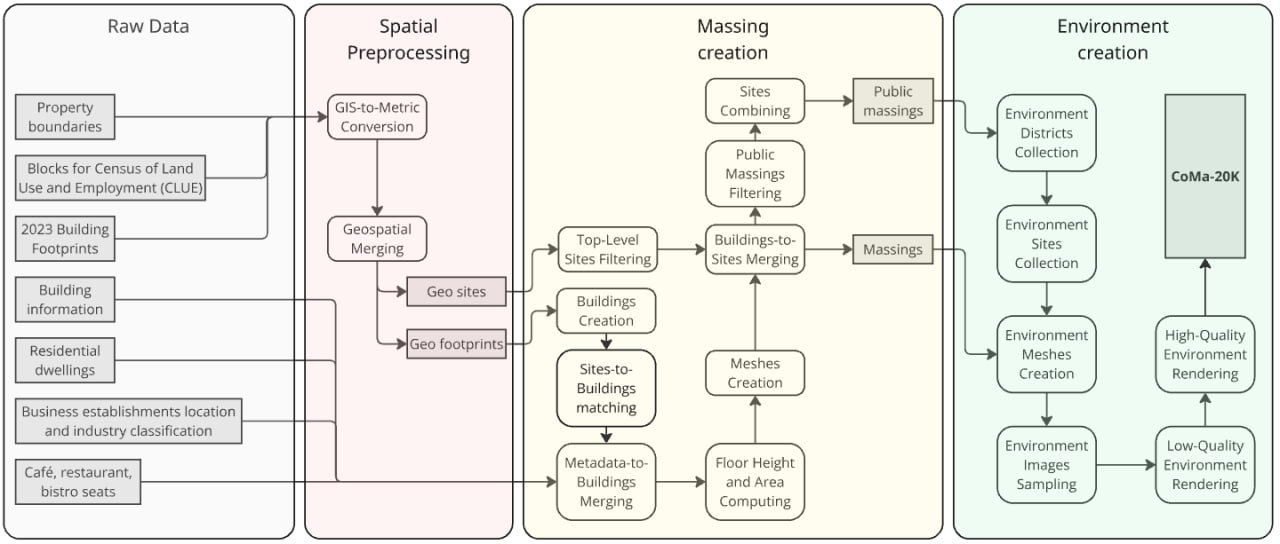
\includegraphics[width=\textwidth]{./images/data_pipeline.jpeg}
    \caption{Dataset Creation Pipeline. The pipeline for constructing the CoMa-20K dataset consists of three main stages: Spatial Preprocessing, where raw geospatial data is converted to a metric system and prepared for merging; Massing Creation, where building geometries are assembled and fused with their functional-economical metadata; and Environment Creation, where the visual context for each site is generated by assembling neighboring buildings and producing multi-style renderings.}
    \label{fig:data_pipeline}
\end{figure*}



The CoMa-20K dataset is constructed entirely from open data provided by the City of Melbourne via their public data platform \cite{melbourne}. This rich source provides a cohesive, real-world foundation for urban modeling. From the approximately 200 available datasets, we selectively utilized seven key tables that, when combined, provide the geometric, contextual, and programmatic information required for our task. The integration of these tables allows us to move from raw civic data to a structured dataset for generative AI.

The data synthesis process revolves around the development site, defined by property boundaries. The following tables were used, with their roles detailed below:

\begin{itemize}
    \item \textbf{Property Boundaries:} This table serves as the foundational layer for the entire dataset. It provides the unique site identifier (\texttt{id}) and the precise polygonal \texttt{site\_contour} for each development lot. All other data is aggregated and associated with these defined sites.

    \item \textbf{2023 Building Footprints:} This table supplies the raw geometric data for constructing the 3D massing models and the surrounding urban context. It contains individual footprint polygons, each with an extrusion height. As these footprints lack a direct property identifier, they are spatially joined to the \texttt{site\_contour} to assemble complete building massings and to the \texttt{CLUE} blocks to build the environmental context.

    \item \textbf{Blocks for Census of Land Use and Employment (CLUE):} These polygons define small statistical districts within the city. We use them as a practical spatial unit to sample the immediate surrounding environment of a target site, ensuring the contextual views are representative of the local urban fabric.
\end{itemize}

The following tables are linked directly to a development site via a shared property ID, enabling the compilation of the functional and economical \texttt{requirements}:

\begin{itemize}
    \item \textbf{Building Information:} This is a primary source for key architectural attributes, providing data such as \texttt{building\_name}, \texttt{n\_floors}, \texttt{building\_function}, and \texttt{floor\_height} for structures on a given property.

    \item \textbf{Residential Dwellings:} For buildings with a residential function, this table provides the crucial \texttt{n\_dwellings} attribute, detailing the number of living spaces (e.g., apartments, houses) within a building on a specific property.

    \item \textbf{Business Establishments Location and Industry Classification:} This table is used to populate the \texttt{offices} list within the requirements. It provides a record of commercial tenants within a building, including their \texttt{name} and business \texttt{function}.

    \item \textbf{Café, Restaurant, Bistro Seats:} Despite its name, this table catalogs a wide range of \texttt{public\_spaces} with known public capacity. It provides the \texttt{name}, \texttt{function}, \texttt{indoor\_capacity}, and \texttt{outdoor\_capacity} for venues like cafes, restaurants, and bars located on a property.
\end{itemize}

\subsection{Dataset Collection Pipeline}

The construction of the CoMa-20K dataset from the raw open data sources is a multi-stage process. This pipeline transforms disparate geospatial and tabular data into a cohesive, multi-modal dataset suitable for training vision-language models. The entire procedure can be divided into three sequential stages: Spatial Preprocessing, Massing Creation, and Environment Creation.

\subsubsection*{Spatial Preprocessing}
This initial stage prepares the raw geospatial data for subsequent geometric operations and merging.

\begin{itemize}
    \item \textbf{GIS-to-Metric Conversion:} All polygon-based datasets (Property Boundaries, Building Footprints, CLUE Blocks), which are originally provided in longitude-latitude coordinates (EPSG:4326), are projected into a local metric coordinate system. This conversion is critical for performing accurate area calculations and spatial intersections.
    \item \textbf{Geospatial Merging:} To link datasets that lack a common identifier (e.g., linking Footprints to Property Boundaries), an all-to-all spatial intersection is computed. To ensure robustness against numerical errors, we do not use a simple binary intersection. Instead, we calculate the actual area of intersection, using this as a reliable metric for establishing relationships between polygons.
\end{itemize}

\subsubsection*{Massing Creation}
This core stage focuses on constructing the 3D building massings and associating them with their functional-economical requirements.

\begin{itemize}
    \item \textbf{Top-Level Sites Filtering:} The Property Boundaries dataset contains nested sites (e.g., a private lot within a larger development). We filter to retain only the top-level, physically distinct development sites to avoid duplication and ensure each site represents a coherent area for development.
    \item \textbf{Buildings Creation:} Individual footprint extrusions from the Building Footprints table are merged together based on spatial proximity to form complete building massings.
    \item \textbf{Sites-to-Building Matching:} Each constructed building is matched to its corresponding development site. A building is assigned to a site if the area of intersection between the building's footprint and the site polygon constitutes over 90\% of the building's total footprint area, ensuring a strong and unambiguous spatial relationship.
    \item \textbf{Metadata-to-Buildings Merging:} Using the established site-to-building links, we merge all metadata from the Building Information, Residential Dwellings, Business Establishments, and Public Spaces tables via their shared property ID. This aggregated data forms the comprehensive \texttt{requirements} dictionary for each building.
    \item \textbf{Floor Height and Area Computing:} Key physical parameters are calculated directly from the geometry. The mean \texttt{floor\_height} is derived from the extrusion data and the number of floors. The \texttt{usable\_area} is computed as the sum of the areas of all horizontal extrusions (floors) within the building massing.
    \item \textbf{Meshes Creation:} The geometric data for each building is compiled into a standard 3D mesh format for rendering and visualization.
    \item \textbf{Buildings-to-Sites Merging:} The finalized buildings, now with their complete geometry and requirements, are grouped back together by their associated site to form the core \texttt{massing} and \texttt{requirements} lists for each dataset sample.
    \item \textbf{Public Massings Filtering:} To focus on larger-scale development, we filter out private houses and townhouses, retaining only public-facing properties such as apartment complexes and commercial offices.
    \item \textbf{Sites Combining:} To increase dataset diversity and include sites with multiple buildings, we programmatically combine 2 to 4 neighboring properties into larger, aggregated development sites.
\end{itemize}

\subsubsection*{Environment Creation}

\begin{figure*}[t]
    \centering
    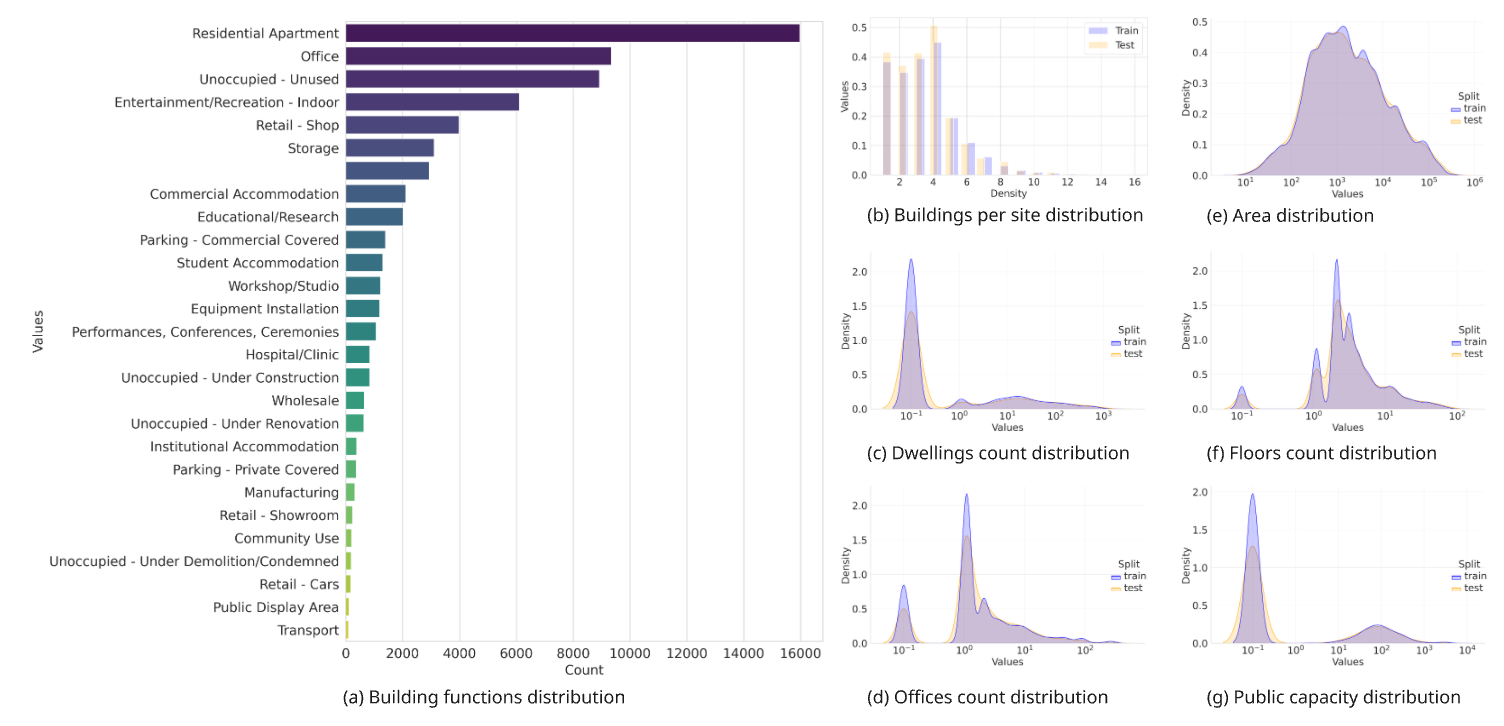
\includegraphics[width=\textwidth]{./images/dataset_stats.png}
    \caption{CoMa-20K Dataset Statistics. Distributions of key attributes across the dataset: (a) building functions, (b) number of buildings per site, (c) dwelling units per building, (d) commercial spaces per building, (e) total usable area, (f) number of floors, and (g) public capacity of commercial spaces.}
    \label{fig:dataset_stats}
\end{figure*}


This final stage generates the crucial contextual visual data for each development site.

\begin{itemize}
    \item \textbf{Environment Districts Collection:} For each target site, we identify its parent CLUE block and all immediately adjacent (neighboring) blocks. Adjacency is determined by a boundary intersection, ensuring a zero-area touch.
    \item \textbf{Environment Sites Collection:} All development sites located within these identified environment districts (parent and neighbors) are collected to form the ``context'' for the target site.
    \item \textbf{Environment Meshes Creation:} A unified 3D environment mesh is created for each target site by concatenating the meshes of all buildings within the collected environment sites.
    \item \textbf{Environment Images Sampling:} Single view for each environment mesh is generated. The target site's contour is overlaid in red for visibility. The camera pose is optimized to maximize the number of pixels occupied by the target site, ensuring it is prominently visible in the context. In parallel, top-down \texttt{map\_image} views are sampled with the site polygon highlighted in two different cartographic styles.
    \item \textbf{Low-Quality Environment Rendering:} The raw environment mesh view is passed through the \textit{Qwen-Image-Edit} \cite{qweni} model to semantically enhance the scene by adding realistic elements like roads and parks, producing a low-realism city environment image (\texttt{env\_render\_low}).
    \item \textbf{High-Quality Environment Rendering:} The low-quality render is fed again into the same image editing model with a prompt for photorealism, resulting in the final, high-detail contextual visualization (\texttt{env\_render\_high}).
\end{itemize}

\subsection{Statistics and Splitting}
  
The final CoMa-20K dataset comprises 20,000 unique development sites, each with associated massings, requirements, and contextual imagery. To facilitate robust model training and evaluation, the dataset was randomly split into a training/validation set (90\%, 18,000 samples) and a held-out test set (10\%, 2,000 samples). This ensures that the model is evaluated on a statistically representative sample of the data that it did not see during training.

An analysis of the dataset reveals several key distributions that characterize the urban fabric of Melbourne as captured in our data:

\begin{itemize}
    \item \textbf{Building Function:} The most prevalent building type is ``Residential Apartment,'' reflecting the city's dense urban core.
    \item \textbf{Buildings per Site:} The majority of development sites contain between 1 and 4 distinct buildings, with single-building sites being the most common.
    \item \textbf{Dwelling Units:} While the mode is a single dwelling unit per building (corresponding to many commercial or small-scale structures), there is a significant secondary mode of buildings containing between 10 and 50 units, representative of mid-rise apartment complexes.
    \item \textbf{Commercial Spaces:} The number of offices or commercial spaces within a building is generally low, with most buildings containing fewer than 5. However, the distribution has a long tail, extending up to approximately 100 for large commercial towers.
    \item \textbf{Total Building Area:} The distribution of \texttt{usable\_area} is right-skewed, with a concentration of buildings around 1,000 m\textsuperscript{2} and a long tail of larger structures.
    \item \textbf{Building Height:} The number of floors is heavily concentrated in low-rise buildings (less than 10 floors), with a small but significant number of high-rise buildings present in the dataset.
    \item \textbf{Public Capacity:} For the subset of buildings that have this data, the public capacity (sum of \texttt{indoor\_capacity} and \texttt{outdoor\_capacity}) is typically distributed around 100 people per building.
\end{itemize}

Detailed distributions for these and other attributes are provided in Figure~\ref{fig:dataset_stats}, which offers a comprehensive visual summary of the dataset's composition.
